% Szglab4
% ===========================================================================
%
\chapter{Analízis modell kidolgozása 1}

\thispagestyle{fancy}

\section{Objektum katalógus}

\subsection{Tower}
Egy tornyot valósít meg. Ha egy ellenség a hatókörébe ér, akkor elindít egy \textbf{Projectile}-t az irányába, a tüzelési gyakoriságának megfelelő időközönként. Ha több ellenfél van a hatókörében, akkor arra lő, aki a legközelebb van a célhoz.

\subsection{Obstacle}
Egy akadályt valósít meg. Ha egy ellenség belelép egy olyan mezőbe, amin van egy \textbf{Obstacle}, akkor azt egy bizonyos mértékben lelassítja, az ellenség fajától függően.

\subsection{Map}
A Map a pályát képviseli, melyben NxM darab cella van. A pálya egy külső fájlból betölthető, ami új játék indulásakor fog megtörténni, miután kiválasztja a játékos a pályát. A pálya különböző tulajdonságai is lekérdezhetőek, amelyek majd a kirajzoláshoz kellenek.

\subsection{Tile}
A Tile objektumból egy NxM -es tömböt fog tárolni a Map objektum. Ezek a pálya egyes celláit fogják képviselni. Egy cellán lehet maximum egy darab épület, amely vagy egy torony, vagy egy akadály, attól függően, hogy van-e a cellán út, vagy nincsen. A cellán levő épület referenciája lekérhető, vagy ha még nincsen rajta, és a cellára kattintás történik, akkor épül egy megfelelő épület.\\
Ha egy cellán van út, akkor lekérdezhető, hogy az a cella milyen távol van a céltól (az utat követve, cellákban mérve). Továbbá az is tárolva van, és lekérdezhető, hogy az út merre folytatódik (és az ellenségeknek merre kell majd menniük). Ha elágazás van, akkor véletlenszerűen választ irányt és arra küldi az ellenséget (ez minden egyes ellenségre véletlenszerű).

\subsection{Mission}
Egy Mission objektumban lesz eltárolva, hogy milyen ellenségek, mikor és honnan jönnek be a pályára. Ez a három adat majd egy segéd osztályban lesz összefogva, és egy tárolóban lesz tárolva. A játék főciklusa le tudja majd kérdezni a következő ellenséget, melyet az objektum visszaad, ha már elég idő eltelt az előző egység óta (ha nem akkor nem ad vissza egységet).

\subsection{Game}
Ez a játék logikáját magába foglaló osztály. Számon tartja a pályán lévő ellenfeleket, akadályokat és tornyokat, valamint végrehajtja a kiválasztott misszió által leírt forgatókönyvet, ami alapján az ellenségek érkeznek.

\subsection{EnemyType}
Leírja egy ellenségtípus (jelen esetben a négy faj: ember, tünde, törp vagy hobbit) tulajdonságait, mint például az alapsebessége és a kezdeti életereje. Minden ellenségnek van egy referenciája egy példányára, amely meghatározza a viselkedését.

\subsection{Enemy}
Az Enemy osztály példányai egy-egy ellenséget tárolnak. Rendelkeznek típussal (fajjal), pillanatnyi pozícióval, hátralévő életerővel. Az idő haladtával próbálnak végighaladni egy véletlenszerűen választott lehetséges útvonalon.

\subsection{Projectile}
Ez a class egy lövedék leírása. Amikor egy torony lő, akkor példányosítja ezt az osztályt a cél ellenség átadásával, így egy lövedék mindig a torony által meghatározott ellenség után megy, amit ha megfelelően megközelít (eltalálja az ellenséget), akkor levesz az életerejéből és megsemmisíti magát.

\subsection{Gem}
Egy épületekre rakható varázskő tulajdonságait tárolja. A Game class fog példányokat létrehozni belőle, különböző tulajdonságokkal. Ha egy épületre rá van rakva egy fajta varázskő, akkor az épület egy referenciát tárol a példányára.


\section{Statikus struktúra diagramok}
\comment{Az előző alfejezet osztályainak kapcsolatait és publikus metódusait bemutató osztálydiagram(ok). Tipikus hibalehetőségek: csillag-topológia, szigetek.}

\begin{figure}[h]
\begin{center}
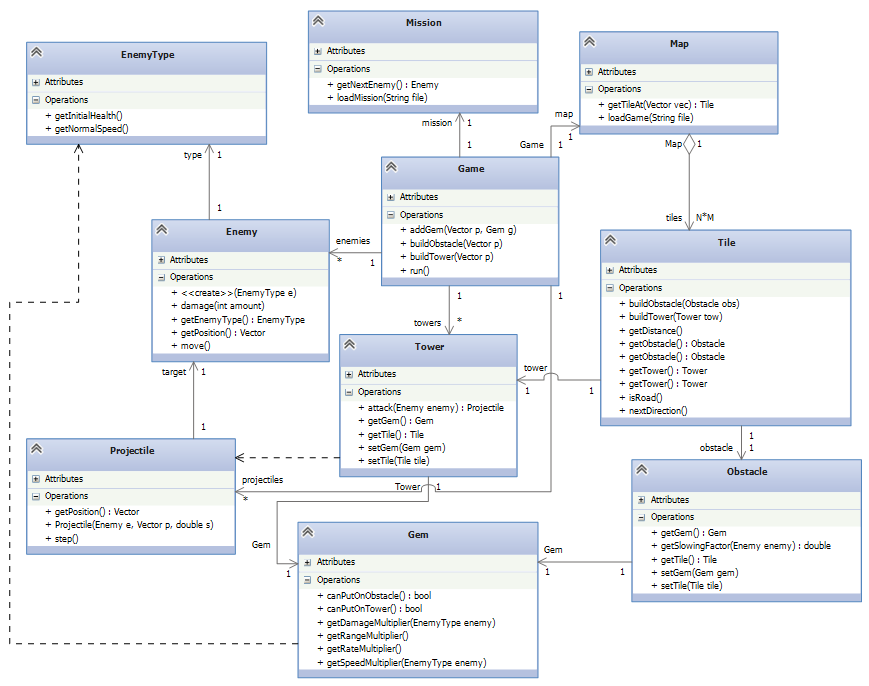
\includegraphics[width=17cm]{images/class.png}
\caption{Osztálydiagram}
\label{fig:class_diag}
\end{center}
\end{figure}


\section{Osztályok leírása}

\subsection{Tower}
\begin{itemize}
\item Felelősség\\
Felelős \textbf{Projectile}-ok létrehozásához, azok megfelelő felparaméterezésével. Továbbá felelős azért, hogy \textbf{Projectile}-okat csak a megadott időközönként lőjjön ki.
\item Attribútumok
	\begin{itemize}
		\item \underline{int cost}: A torony ára varázserőben.
		\item gem: Eltárol egy referenciát egy \textbf{Gem} típusú objektumra, ami meghatározza, hogy az adott épület milyen echant alatt áll.
		\item Map<EnemyType, double> damage: Megadja mekkora az adott típusú ellenfélre kifejtett hatása a toronynak.
		\item \textbf{Tile} tile: Egy referencia arra a mezőre, ahol az épület található.
	\end{itemize}
\item Metódusok
	\begin{itemize}
		\item \textbf{Projectile} attack(\textbf{Enemy} enemy): Kilő egy \textbf{Projectile}-t a paraméterként megkapott ellenségre, majd a visszatérési értékében visszaadja azt. A \textbf{Projectile}-t felparaméterezi az ellenséghez megfelelő sebzési adatokkal.
		\item \textbf{Gem} getGem(): Visszaadja az épületen található varázskövet.
		\item void setGem(\textbf{Gem} gem): Beállítja az epületen lévő varázskövet. Ha már volt az épületen varázskő, akkor az előző megszűnik.
		\item void setTile(\textbf{Tile} tile): Beállítja, hogy a torony melyik \textbf{Tile}-on van.
		\item \textbf{Tile} getTile(): Visszaadja, hogy a torony melyik \textbf{Tile}-on van.
	\end{itemize}
\end{itemize}


\subsection{Obstacle}
\begin{itemize}
\item Felelősség\\
Felelős \textbf{Projectile}-ok létrehozásához, azok megfelelő felparaméterezésével. Továbbá felelős azért, hogy \textbf{Projectile}-okat csak a megadott időközönként lőjjön ki.
\item Attribútumok
		\item \underline{int cost}: Az akadály ára varázserőben.
		\item Gem gem: Eltárol egy referenciát egy \textbf{Gem} típusú objektumra, ami meghatározza, hogy az adott épület milyen echant alatt áll.
		\item Map<EnemyType, double> speedMultiplier: Megadja mekkora az adott típusú ellenfélre kifejtett hatása az akadálynak.
		\item \textbf{Tile} tile: Egy referencia arra a mezőre, ahol az épület található.
\item Metódusok
	\begin{itemize}
		\item double getSlowingFactor(\textbf{Enemy} enemy): Visszatér azzal az értékkel, amivel az adott ellenfelet lassítja.
		\item \textbf{Gem} getGem(): Visszaadja az épületen található varázskövet.
		\item void setGem(\textbf{Gem} gem): Beállítja az epületen lévő varázskövet. Ha már volt az épületen varázskő, akkor az előző megszűnik.
		\item void setTile(\textbf{Tile} tile): Beállítja, hogy az akadály melyik \textbf{Tile}-on van.
		\item \textbf{Tile} getTile(): Visszaadja, hogy az akadály melyik \textbf{Tile}-on van.
	\end{itemize}
\end{itemize}


\subsection{Map}
\begin{itemize}
\item Felelősség\\
Tartlamaz az összes cellára referenciát, felelős a kapott fájlból beolvasni a pályát, és felépíteni azt.
\item Attribútumok
	\begin{itemize}
		\item Tile[][] tiles: A pályán található cellák tömbje, a pálya kirajzolásához használható.
	\end{itemize}
\item Metódusok
	\begin{itemize}
		\item Tile getTileAt(Vector position): Visszaadja a position helyen talalható cellát.
		\item loadGame(String file): Betölti a kapott elérési útvonalon a fájlt, és felépíti az alapján a pályát.
	\end{itemize}
\end{itemize}


\subsection{Mission}
\begin{itemize}
\item Felelősség\\
Felelőssége, felépíteni a listát, amely a beérkező ellenségeket és időzítésüket tartalmazza. Majd a megfelelő időközönként ki kell adja ezeket az egységeket a Game osztálynak.
\item Attribútumok
	\begin{itemize}
		\item List<Spawn> spawnList: A Spawn segédosztályban tárolt ellenség-idő-belépési pont, adatokat tárolja.
		\item double lastSpawn: Tárolja az előző spawn idejét.
	\end{itemize}
\item Metódusok
	\begin{itemize}
		\item Enemy getNextEnemy(double time): A spawnList listaból a következő elemet megvizsgaálja, és ha spawnolni kell a következő ellenséget, akkor visszaadja azt.
		\item loadMission(String file): Betölti a kapott elérési útvonalon a fájlt, és felépíti az alapján a listát (spawnList).
	\end{itemize}
\end{itemize}


\subsection{Tile}
\begin{itemize}
\item Felelősség\\
Egy cellán lehet maximum egy darab épület, amely vagy egy torony, vagy egy akadály, attól függően, hogy van-e a cellán út, vagy nincsen. A cellán levő épület referenciája lekérhető, vagy ha még nincsen rajta, és a cellára kattintás történik, akkor épül egy megfelelő épület. Felelős még az egyes ellenségek következő irányának a meghatározására, és vissza kell tudnia adni, hogy van-e rajta út, valamint ha van akkor milyen távol van a céltól.
\item Attribútumok
	\begin{itemize}
		\item Building building: A cellában levő epület.
		\item int distance: Hányadik cella az utat követve a céltól.
		\item bool road: Van-e út a cellában.
		\item double up: Annak a valószinűsége, hogy a cellából felfelé fog menni az ellenség.
		\item double down: Annak a valószinűsége, hogy a cellából lefelé fog menni az ellenség.
		\item double left: Annak a valószinűsége, hogy a cellából balra fog menni az ellenség.
		\item double right: Annak a valószinűsége, hogy a cellából jobbra fog menni az ellenség.
	\end{itemize}
\item Metódusok
	\begin{itemize}
		\item void buildTower(): A cellán egy tornyot épít.
		\item void buildObstacle(): A cellán egy akadályt épít.
		\item Tower getTower(): Visszaadja a cellán lévő tornyot.
		\item Obstacle getObstacle(): Visszaadja a cellán lévő akadályt.
		\item int getDistance(): Visszaadja a distance értékét.
		\item bool isRoad(): Visszaadja a road értékét.
		\item Direction nextDirection(): Visszad egy irány enum-ot, amely megadja az ellenség irányát.
	\end{itemize}
\end{itemize}


\subsection{Game}
\begin{itemize}
\item Felelősség\\
A többi osztály nyilván tartása és összekötése, a játékbeli események vezérlése. A felhasználói felülettől érkező parancsok végrehajtása, és a játék állapotának rendelkezésre bocsájtása a kijelzéshez.
\item Attribútumok
	\begin{itemize}
		\item ArrayList<Projectile> projectiles: Eltárolja a jelenleg játékban lévő lövedékeket.
		\item Map map: Referencia a kiválasztott pályára, amin a játék folyik.
		\item Mission mission: Referencia a kiválasztott misszióra, amely alapján zajlik a játék.
		\item ArrayList<Building> buildings: Eltárolja a játékos megépített tornyait.
		\item ArrayList<Gem> gems: Az összes lehetséges, toronyra illetve akadályra rakható varázskő nyilvántartása.
		\item ArrayList<EnemyType> types: Ez a lehetséges ellenségtípusok listája.
		\item ArrayList<Enemy> enemies: Az összes éppen látható ellenség található meg benne.
		\item int magic: A játékos jelenlegi varázsereje.
	\end{itemize}
\item Metódusok
	\begin{itemize}
		\item void run(): Ez a metódus futtatja a főciklust, amelyben maga a játék működik.
		\item void buildTower(Vector position): Épít egy tornyot a paraméterül kapott helyen évő mezőre.
		\item void buildObstacle(Vector position): Épít egy akadályt a paraméterül kapott helyen lévő mezőre.
		\item void addGem(Vector position, Gem gem): A paraméterként kapott helyen lévő toronyra vagy akadályra rárakja a paraméterként kapott varázskövet.
		\item \comment{\textbf{TODO}, ez még hiányos.}
	\end{itemize}
\end{itemize}


\subsection{EnemyType}
\begin{itemize}
\item Felelősség\\
Leírja egy bizonyos típusú (fajú) ellenség alapvető tulajdonságait. Egy-egy példányára hivatkozik az összes ellenség, amelyeknek ezáltal meghatározza a viselkedését.
\item Attribútumok
	\begin{itemize}
		\item int cost: Az ilyen fajtájú ellenségek ára varázserőben.
		\item double initialHealth: Az ilyen fajtájú ellenségek kezdeti életereje.
		\item double normalSpeed: Az ilyen fajtájú ellenségek akadályoztatás nélküli haladási sebessége.
	\end{itemize}
\item Metódusok
	\begin{itemize}
		\item double getInitialHealth(): Visszaadja az initialHealth attribútum értékét.
		\item double getNormalSpeed(): Visszaadja a normalSpeed attribútum értékét.
	\end{itemize}
\end{itemize}


\subsection{Enemy}
\begin{itemize}
\item Felelősség\\
Az ellenségek pozíciójának, sebességének és életerejének nyilvántartása.
\item Attribútumok
	\begin{itemize}
		\item EnemyType type: Az egység típusa.
		\item double health: Az ellenség fennmaradó életereje.
		\item Vector position: Pillanatnyi pozíció a pályán.
	\end{itemize}
\item Metódusok
	\begin{itemize}
		\item boolean move(double dt): Az egységet annyival mozgatja az útján tovább, amennyit dt idő alatt halad. Ha az ellenség életereje 0 vagy kisebb, akkor true-val tér visza, egyébként false-al.
		\item Vector getPosition(): A position attribútum értékével tér vissza.
		\item bool damage(double amount): Csökkenti az ellenség életerejét amount-al, igazzal tér vissza ha az ellenség meghalt.
		\item EnemyType getEnemyType(): Visszaadja az ellenség típusát.
	\end{itemize}
\end{itemize}


\subsection{Projectile}
\begin{itemize}
\item Felelősség\\
Követni a cél ellenséget, majd sebezni ha eléri.
\item Attribútumok
	\begin{itemize}
		\item double damage: A lövedék sebzése, ennyivel csökkenti a cél ellenség életerejét amikor eltalálja.
		\item Vector position: A lövedék pozíciója.
		\item double speed: A lövedék sebessége.
		\item Enemy enemy: A lövedék cél Enemy-je.
	\end{itemize}
\item Metódusok
	\begin{itemize}
		\item Projectile(Enemy enemy, Vector position, double speed): Konstruktor, átveszi a cél Enemy-t, a kezdő pozíciót és sebességet.
		\item boolean move(double dt): dt * speed-el mozgatja a lövedéket az ellenség irányába. Ha eltalálta az ellenséget vagy az ellenség már meghalt, akkor true-t ad vissza, különben false-t.
		\item Vector getPosition(): Visszaadja a lövedék pozícióját.
	\end{itemize}
\end{itemize}


\subsection{Gem}
\begin{itemize}
\item Felelősség\\
Egy fajta varázskő tulajdonságainak tárolása.
\item Attribútumok
	\begin{itemize}
		\item int cost: A varázskő ára varázserőben.
		\item double rangeMultiplier: Megadja, hogy a varázskővel ellátott toronynak hányszorosára nő a hatótávolsága.
		\item double rateMultiplier: Megadja, hogy a varázskővel ellátott toronynak hányszorosára nő a tüzelési sebessége.
		\item HashMap<EnemyType, Double> damageMultiplier: Megadja, hogy a varázskővel ellátott toronynak hányszorosára nő a sebzése egy adott típusú ellenséggel szemben.
		\item HashMap<EnemyType, Double> speedMultiplier: Megadja, hogy a varázskővel elátott akadályon áthaladó adott típusú ellenség sebessége hányadára csökken.
	\end{itemize}
\item Metódusok
	\begin{itemize}
		\item Gem(double rangeMultiplier, double rateMultiplier, HashMap<EnemyType, Double> damageMultiplier, HashMap<EnemyType, Double> speedMzltiplier): Létrehoz egy Gem objektumot a paraméterként kapott tulajdonságokkal.
		\item double getRangeMultiplier(): Visszaadja a varázskő hatótávolság szorzóját.
		\item double getRateMultiplier(): Visszaadja a varázskő tüzelési sebesség szorzójáz.
		\item double getDamageMultiplier(EnemyType enemyType): Visszaadja varázskő sebzés szorzóját egy adott típusú ellenséghez.
		\item double getSpeedMultiplier(EnemyType enemyType): Visszaadja varázskő sebesség szorzóját egy adott típusú ellenséghez.
		\item boolean canPutOnTower(): Ha a varázskő használható tornyokra, igazat ad vissza, különben hamisat.
		\item boolean canPutOnObstacle() Ha a varázskő használható akadályokra, igazat ad vissza, különben hamisat.
	\end{itemize}
\end{itemize}


\section{Szekvencia diagramok}
\comment{Inicializálásra, use-case-ekre, belső működésre. Konzisztens kell legyen az előző alfejezettel. Minden metódus, ami ott szerepel, fel kell tűnjön valamelyik szekvenciában. Minden metódusnak, ami szekvenciában szerepel, szereplnie kell a valamelyik osztálydiagramon.}

\begin{figure}[!h]
\begin{center}
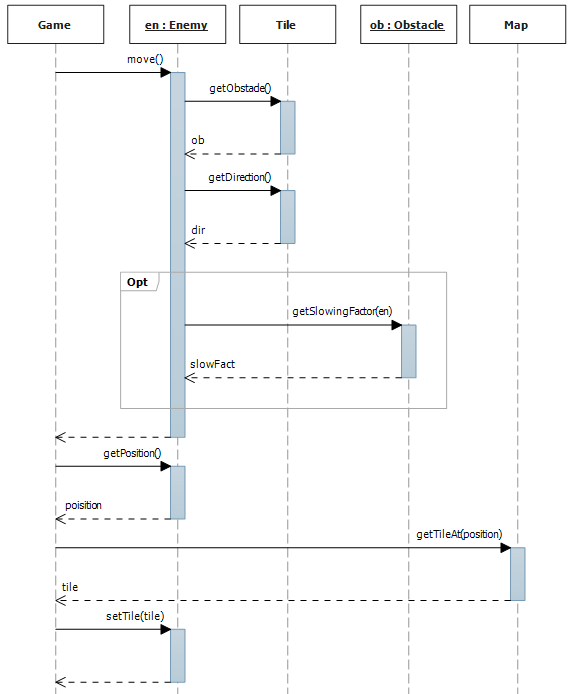
\includegraphics[width=13cm]{images/move_enemy.png}
\caption{Ellenség mozgatása}
\label{fig:move_enemy}
\end{center}
\end{figure}

\begin{figure}[!h]
\begin{center}
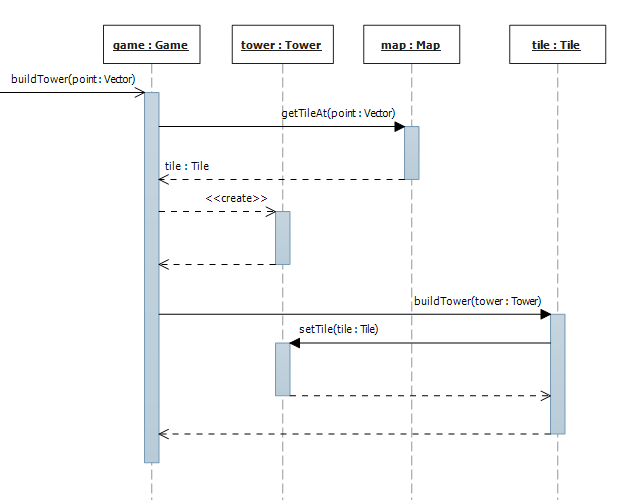
\includegraphics[width=15cm]{images/build_tower.png}
\caption{Torony építése}
\label{fig:build_tower}
\end{center}
\end{figure}

\begin{figure}[!h]
\begin{center}
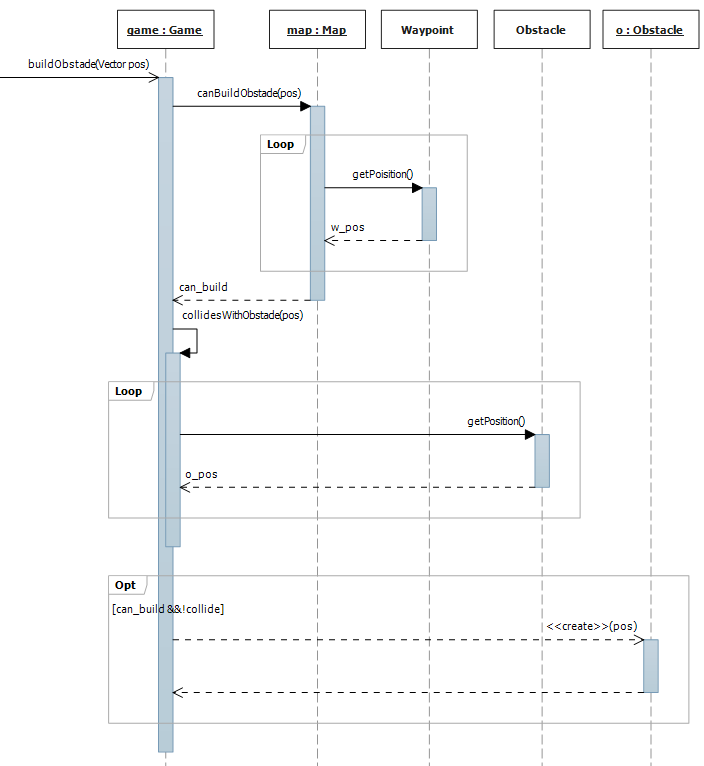
\includegraphics[width=15cm]{images/build_obstacle.png}
\caption{Akadály építése}
\label{fig:build_tower}
\end{center}
\end{figure}

\begin{figure}[!h]
\begin{center}
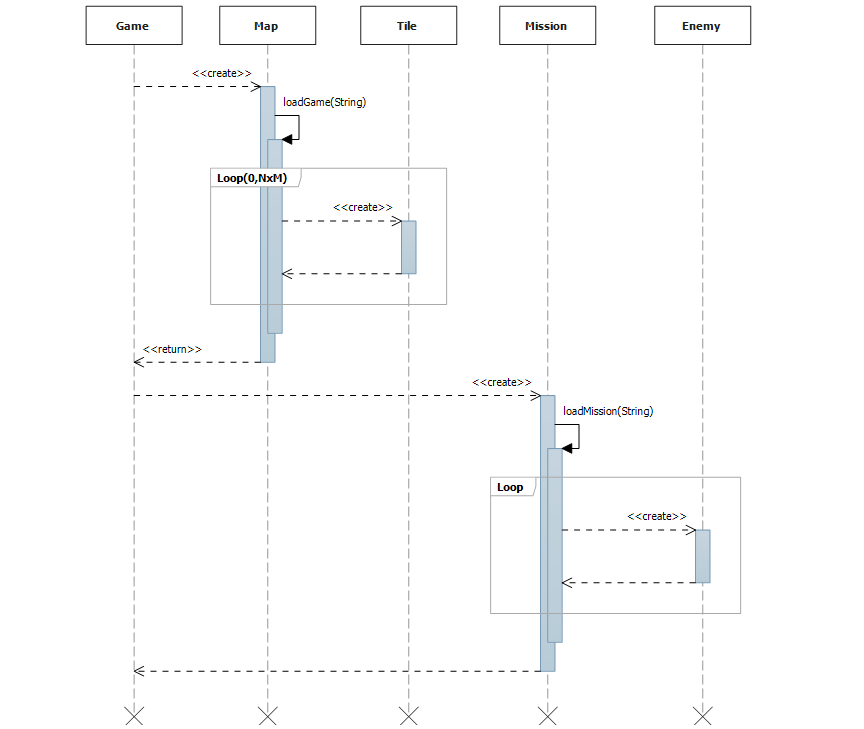
\includegraphics[width=15cm]{images/jatekInditasa.png}
\caption{Játék Indítása}
\label{fig:game_start}
\end{center}
\end{figure}

\begin{figure}[!h]
\begin{center}
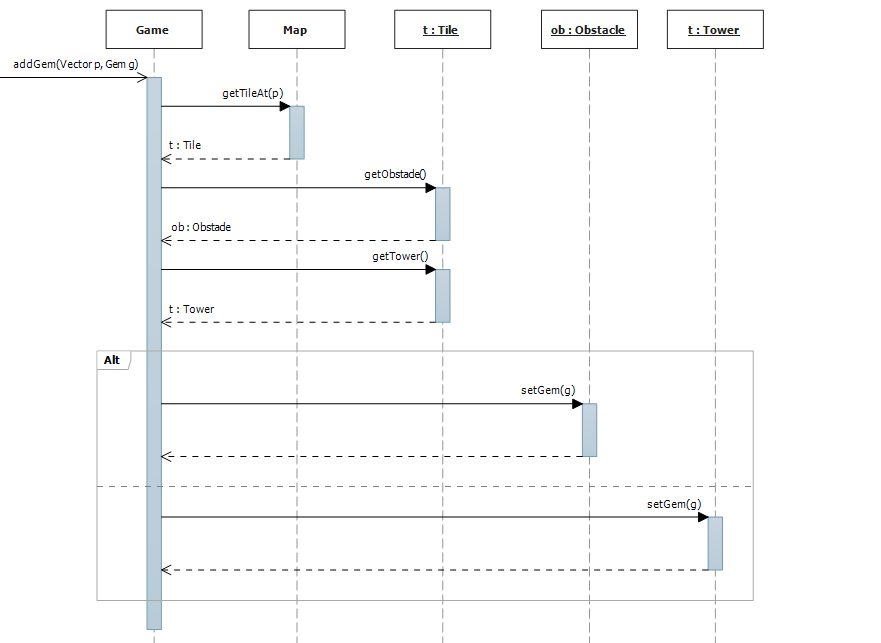
\includegraphics[width=15cm]{images/add_gem.png}
\caption{Varázskő felvétele}
\label{fig:set_gem}
\end{center}
\end{figure}

\pagebreak
\section{State-chartok}
\comment{Csak azokhoz az osztályokhoz, ahol van értelme. Egyetlen állapotból álló state-chartok ne szerepeljenek. A játék működését bemutató state-chart-ot készíteni tilos.}

\begin{figure}[h]
\begin{center}
%\includegraphics[width=17cm]{chapters/chapter03/example.pdf}
\caption{x}
\label{fig:example3}
\end{center}
\end{figure}

